\documentclass[a4paper,11pt,titlepage]{article}

\usepackage{latexsym}
\usepackage{graphicx}
\usepackage{float}
\usepackage{url}
\usepackage{unicode}
\usepackage[polish]{babel}
\usepackage{titlesec}
\usepackage{listings}
\usepackage{xcolor}
\usepackage{setspace}
\usepackage{subfig}
\usepackage{tabularx}
\usepackage{courier}
\DeclareUnicodeCharacter{200B}{{\hskip 0pt}}

\definecolor{codeblue}{rgb}{0,0,0.6}
\definecolor{codegray}{rgb}{0.5,0.5,0.5}
\definecolor{codepurple}{rgb}{0.58,0,0.82}
\definecolor{backcolour}{rgb}{0.96,0.96,0.96}

\lstdefinestyle{code}{
    backgroundcolor=\color{backcolour},
    keywordstyle=\color{codeblue},
    numberstyle=\tiny\color{codegray},
    stringstyle=\color{codeblue},
    basicstyle=\ttfamily\footnotesize,
    breakatwhitespace=false,
    breaklines=true,
    captionpos=b,
    keepspaces=true,
    numbers=left,
    numbersep=3pt,
    showspaces=false,
    showstringspaces=false,
    showtabs=false,
    tabsize=1,
    basicstyle=\small
}

\lstset{style=code}

\newcommand{\sectionbreak}{\clearpage}
\author{Adam Talarczyk}
\title{Symulacje Monte Carlo}
\frenchspacing
\begin{document}
\begin{titlepage}
    \begin{center}

        \Huge
        \textbf{WYDZIAŁ NAUK ŚCISŁYCH I TECHNICZNYCH}
        
        
        \vspace{1.5cm}
	   Symulacje Komputerowe
        \LARGE
        
	\vspace{2cm}
	
	Sprawozdanie ``Symulacja Monte Carlo''

	\vspace{1cm}
	Adam Talarczyk, Mateusz Wrzoł
	
	\vspace{5cm}
        \vfill

        \vspace{0.8cm}
	\Large
        Uniwersytet Śląski, Sosnowiec, 2021

    \end{center}
\end{titlepage}
\newpage

%\tableofcontents
% \newpage


\section{Zadanie 1}
Należy zmodyfikować kod dla aproksymacji stałej $\pi$, aby sprawdzić jak rozmiar próbki wpływa na błąd aproksymacji. Błąd aproksymacji obliczamy jako wartość bezwględną różnicy, pomiędzy aproksymacją $\pi$ i wartością rzeczywistą $\pi$ (3.14159265). Należy przygotować wykres [Rysunek \ref{fig:wykres1}].

\begin{figure}[H]
\centering
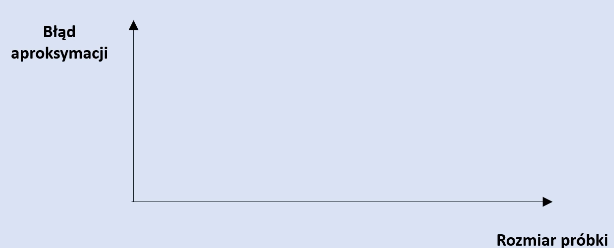
\includegraphics[width=1\columnwidth]{img/zad1.PNG}
\caption{Przykład wykresu}
\label{fig:wykres1}
\end{figure}

\subsection{Rozwiązanie}
Do uzyskania odpowiednich wyników konieczne było wyliczenie aproksymacji $\pi$ dla wielu próbek. W zadaniu wykorzystano próbki z zakresu od 1 do 1000000. Dodatkowo, konieczne było kilkukrotne powtórzenie wykonywanej aproksymacji w celu uśrednienia otrzymanego przybliżenia $\pi$. W opisywanym przykładzie zastosowano 10 powtórzeń. Błąd aproksymacji został wyliczony jako różnica bezwzglęna pomiędzy zdefiniowaną stałą \verb|3,14159265| oraz uzyskanym uśrednionym przybliżeniem. Wyniki zaprezentowane są w tablicy \ref{tab:res}.

\begin{table}[h!]
\centering
\begin{tabular}{ |c|c|c| } 
 \hline
 Próbka & Średnie przybliżenie $\pi$ & Błąd aproksymacji \\
 \hline
 1	& 3,6 &	0,45840735 \\
 10	& 3,04 &	0,10159265 \\
 100	& 	3,064 &	0,07759265 \\
 1000	& 3,124 &	0,01759265 \\
 10000	& 3,13392 &	0,00767265 \\
 100000	& 	3,140084 &	0,00150865 \\
 1000000	& 3,1409996 &	0,00059305 \\
 \hline
\end{tabular}
\caption{Tablica z wynikami uzyskanymi w symulacji}
\label{tab:res}
\end{table}

Na podstawie powyższych danych wygenerowany został wykres za pomocą funkcji \verb|plot()| (Rysunek \ref{fig:pi10}). 

\begin{figure}[H]
\centering
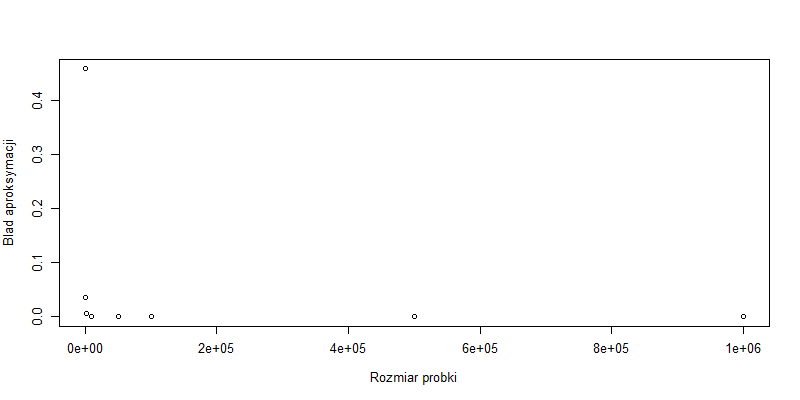
\includegraphics[width=1\columnwidth]{img/pi10.PNG}
\caption{Wygenerowany wykres przedstawiający błąd aproksymacji względem rozmiaru próbki}
\label{fig:pi10}
\end{figure}

Przedstawiony na rysunku \ref{fig:pi10} wykres jest mało czytelny, dlatego wyeksportowano dane do pliku o rozszerzeniu \verb|xlsx| i na ich podstawie utworzono kolejne wykresy: Błąd aproksymacji względem rozmiaru próbki (Rysunek \ref{fig:pie1}) oraz przybliżenie PI względem rozmiaru próbki z zaznaczoną wartością 3,14159265 (Rysunek \ref{fig:pie2}).

\begin{figure}[H]
\centering
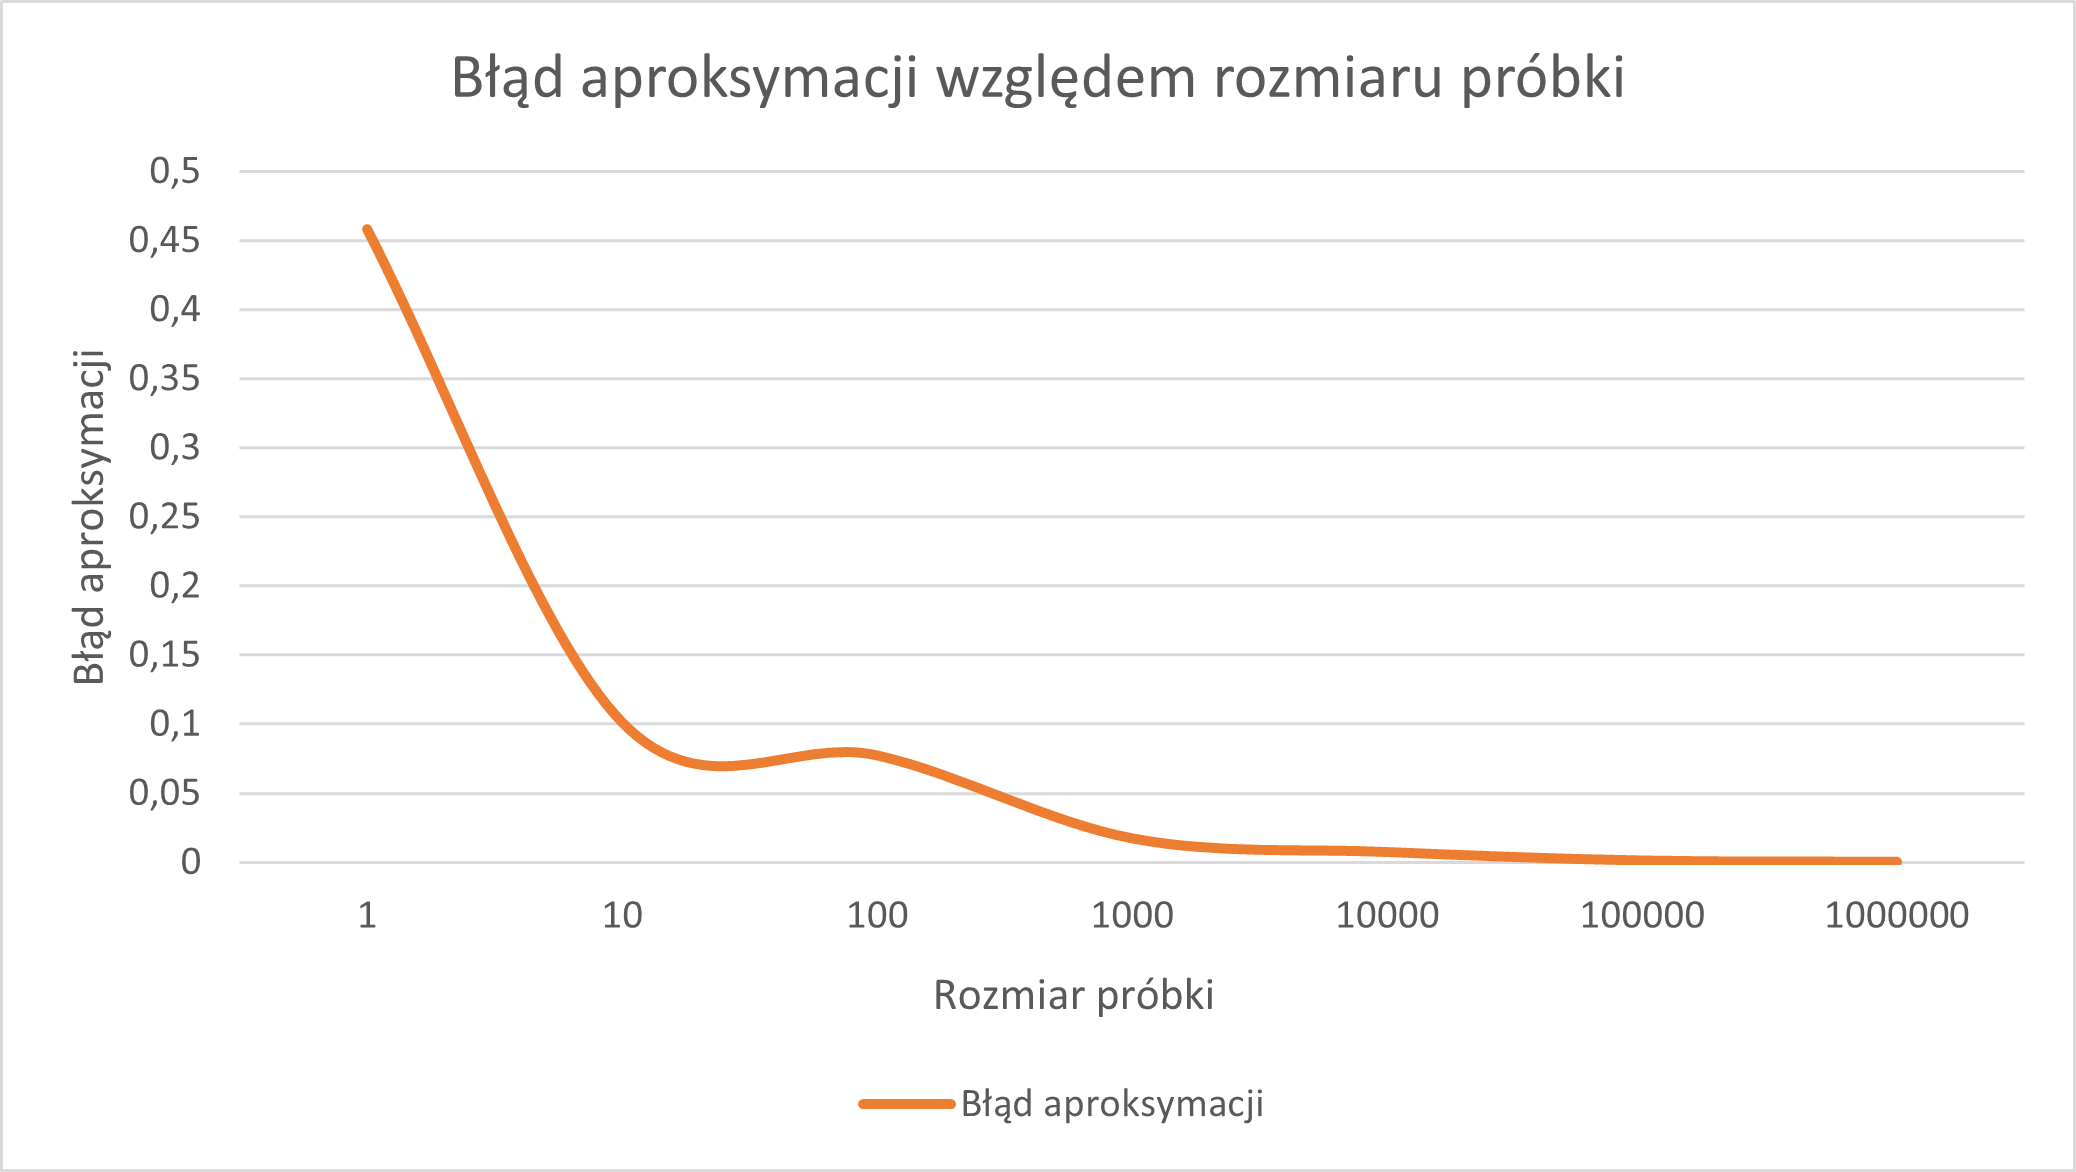
\includegraphics[width=1\columnwidth]{img/pi-excel.PNG}
\caption{Wykres przedstawiający błąd aproksymacji względem rozmiaru próbki}
\label{fig:pie1}
\end{figure}

\begin{figure}[H]
\centering
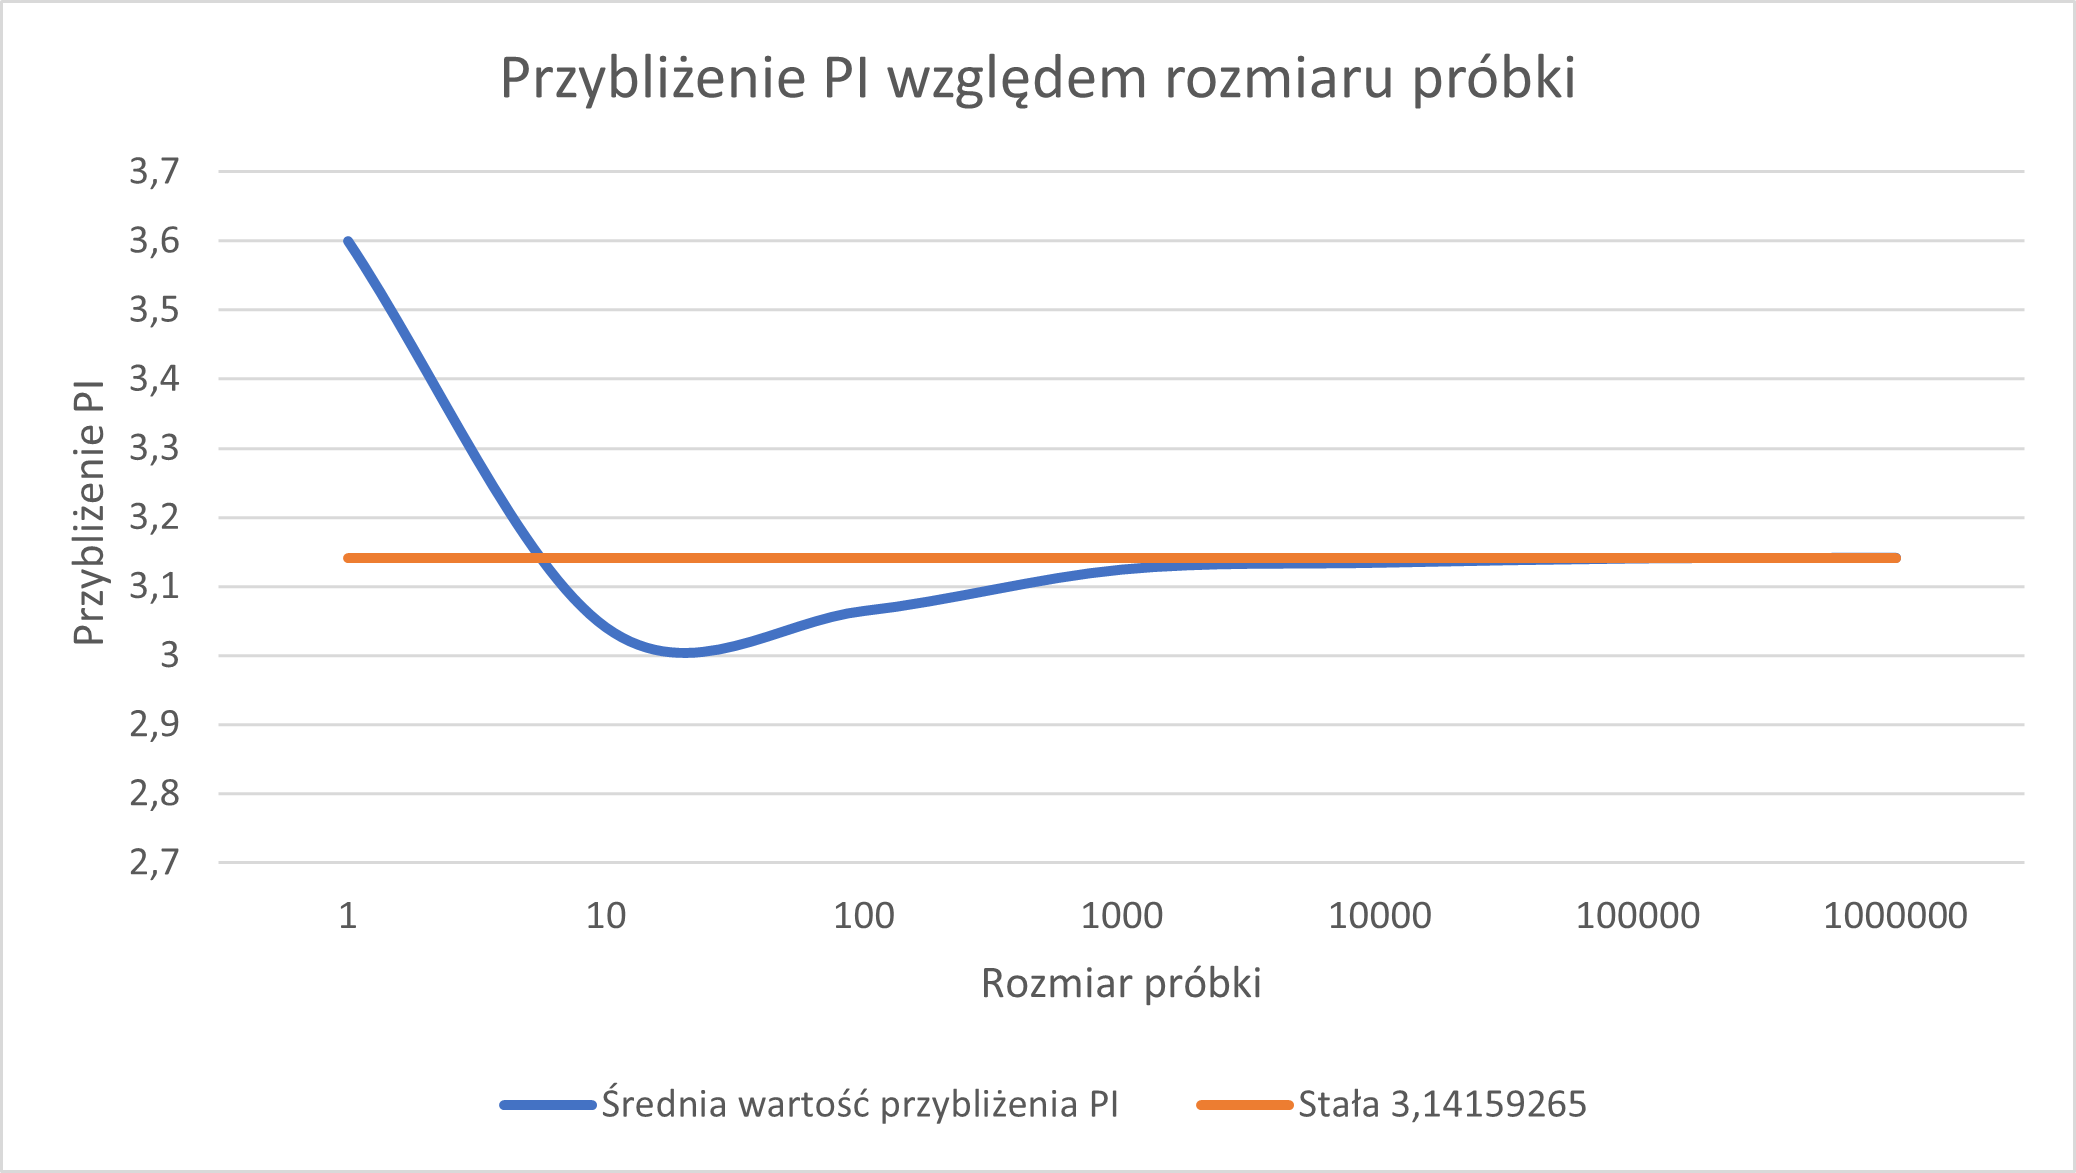
\includegraphics[width=1\columnwidth]{img/pi-excel2.PNG}
\caption{Wykres przedstawiający przybliżenie PI względem rozmiaru próbki, w porównaniu do wartości 3,14159265}
\label{fig:pie2}
\end{figure}

Na podstawie przedstawionej symulacji można stwierdzić, że wielkość błędu aproksymacji zależy od wielkości próbki. Im większa próbka, tym mniejszy jest błąd aproksymacji, a przybliżenie liczby $\pi$ jest bardziej dokładne.

\subsection{Kod źródłowy}
\lstinputlisting[language=R, caption=Plik main.R- wywołanie głównej funkcji, label={main}]{../pi/main.R}
\lstinputlisting[language=R, caption=Plik avarage\_difference.R- odpowiedzialny za wyliczanie błędu aproksymacji PI, label={avg-abs-dif}]{../pi/avarage_difference.R}
\lstinputlisting[language=R, caption=Plik approximation.R- odpowiedzialny za obliczanie przybliżenia liczby $\pi$, label={approx}]{../pi/approximation.R}

\newpage
\section{Zadanie 2}
Zaprogramować symulację Monte Carlo (np. w języku R), która pozwoli obliczyć pole powierzchni szarego obszaru, przedstawionego na poniższym rysunku [Rysunek \ref{fig:wykres2}]. Obliczyć błąd uzyskanego wyniku.

\begin{figure}[H]
\centering
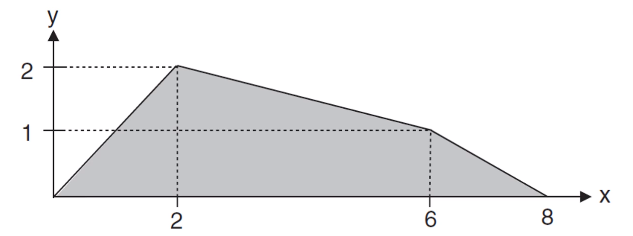
\includegraphics[width=1\columnwidth]{img/zad2.PNG}
\caption{Figura}
\label{fig:wykres2}
\end{figure}

\subsection{Rozwiązanie}
W celu uzyskania odpowiedniego wyniku, w pierwszej kolejności generowane są punkty dla współrzednych \verb|x| (od 0 do 8) i \verb|y| (od 0 do 2). Następnie sprawdzane jest, czy punkty znajdują się w przestrzeni odpowiedniej figury (z podziałem na mniejsze figury, takie jak prawy trójkąt, lewy trójkąt, środkowy trójkąt oraz środkowy prostokąt). Kolejnym krokiem jest połączenie wyników dla poszczególnych figur w jeden wielokąt z treści zadania. Dokładne pole figury zostało wyliczone jako suma poszczególnych elementów wielokąta, zastosowano działanie \verb|(2*2/2)+(1*4/2)+(1*2/2)+(1*4)|, którego wynik wynosi 9. Wynik symulacji to iloraz sumy punków w figurze i liczby wygenerowanych punktów, pomnożony przez pole badanego obszaru (\verb|2*8=16|). Błąd uzyskanego wyniku został wyliczony jako wartość bezwzględna z różnicy uzyskanego wyniku i dokładnego pola figury. Na sam koniec wygenerowany został wykres przy użyciu funkcji \verb|plot()| (Resunek \ref{fig:fig1m}).

\begin{figure}[H]
\centering
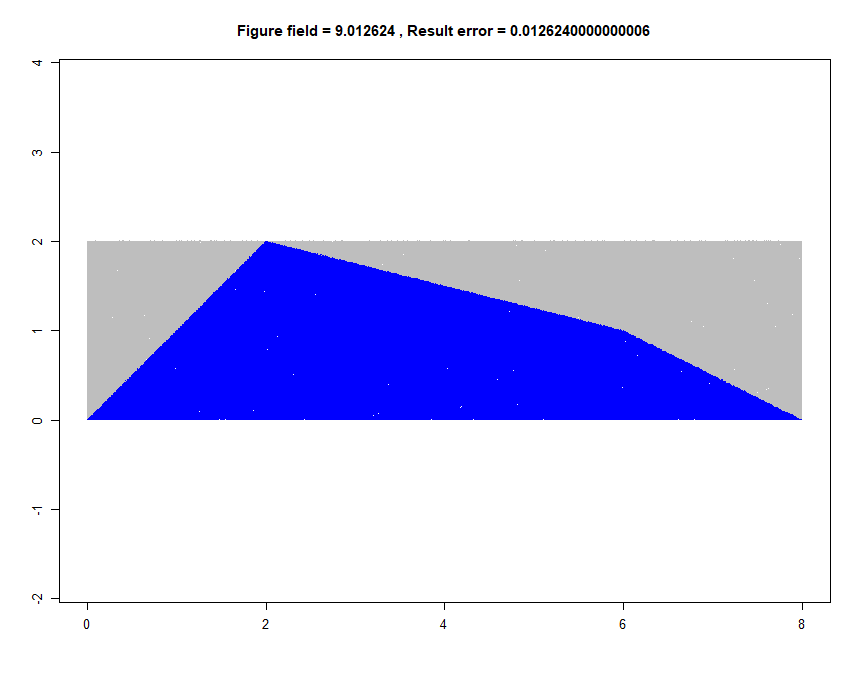
\includegraphics[width=1\columnwidth]{img/figure1m.PNG}
\caption{Figura utworzona przy użyciu funkcji plot() dla próbki równej 1000000}
\label{fig:fig1m}
\end{figure}


Wyniki dla poszczególnych próbek zamieszczone są w tablicy \ref{tab:figwynik}. Dodatkowo, wygenerowane wykresy przedstawione są na rysunku \ref{fig:figs} w formie porównania względem wielkości próbki.

\begin{table}[h!]
\centering
\begin{tabular}{ |c|c|c| } 
 \hline
 Próbka & Pole figury & Błąd \\
 \hline
 100000	& 9.0352 &	0.0351999999999997 \\
 1000000	& 9.012624 & 0.0126240000000006 \\
 \hline
\end{tabular}
\caption{Tablica z wynikami uzyskanymi w symulacji}
\label{tab:figwynik}
\end{table}

\begin{figure}[H]%
    \centering
    \subfloat[\centering Wynik symulacji dla próbki 100000]{{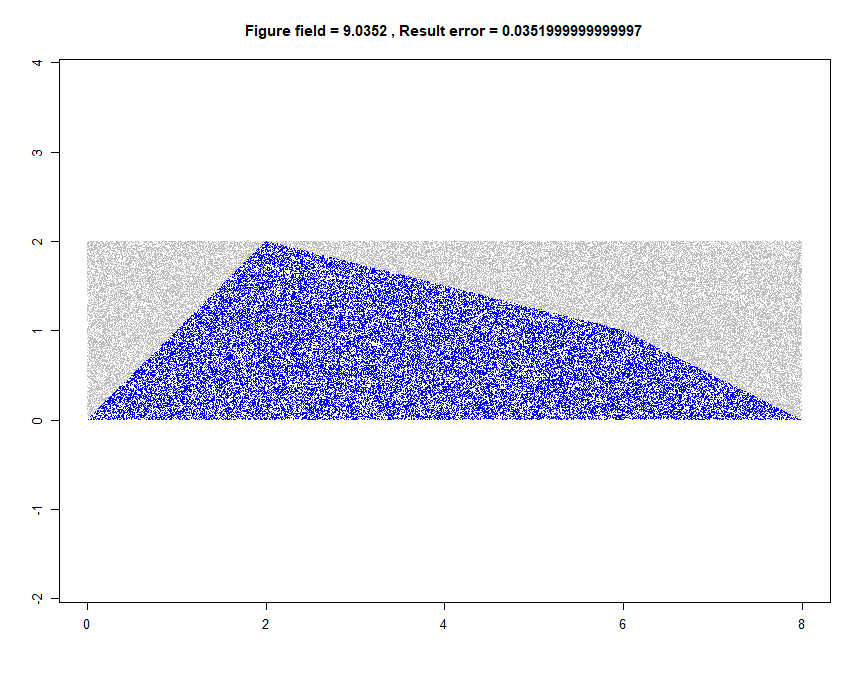
\includegraphics[width=5cm]{img/figure100k.PNG} }}%
    \qquad
    \subfloat[\centering Wynik symulacji dla próbki 1000000]{{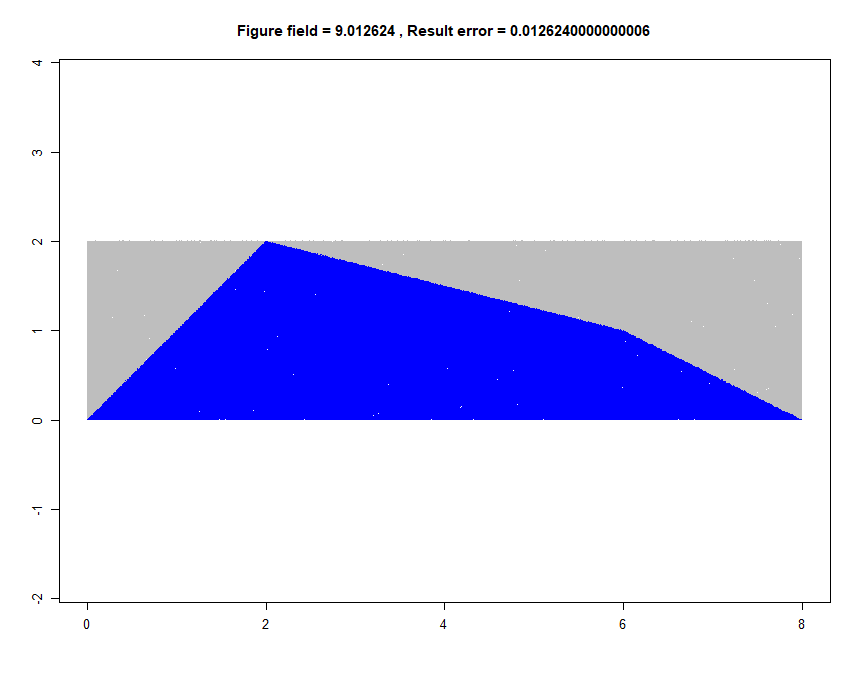
\includegraphics[width=5cm]{img/figure1m.PNG} }}%
    \caption{Porównanie wizualizacji figur pod względem wielkości próbki}%
    \label{fig:figs}%
\end{figure}

Na podstawie przedstawionych wyników zauważyć można, że dokładność uzyskanego pola figury rośnie wraz ze zwiększeniem probki.

\subsection{Kod źródłowy}
\lstinputlisting[language=R, caption=Plik figure.R- odpowiedzialny za obliczenie pola i wygenerowanie wykresu, label={approx2}]{../figure/figure.R}

\end{document}
